
\RequirePackage{plautopatch}  % pLaTeX または upLaTeX のとき
%\documentclass[uplatex,dvipdfmx,titlepage,a4j]{jsarticle}% upLaTeX のとき
\documentclass[dvipdfmx,titlepage,a4j]{jsarticle}  % pLaTeX のとき
\usepackage{listings,jvlisting}
\usepackage{amsmath,amssymb}
\usepackage{graphicx}
\usepackage[yen]{okuverb}
\usepackage{r04ec-exp}
\usepackage{here}
\usepackage{ascmac}
\usepackage{fancybox}
\usepackage{fancyvrb}
\usepackage{fancyhdr}
\usepackage{lastpage}
\usepackage{cases}
\usepackage[hang,small,bf]{caption}
\usepackage[subrefformat=parens]{subcaption}

\fancypagestyle{foot}
{
\fancyhead[C]{OPアンプの基礎・応用}
\fancyfoot[C]{\thepage / \pageref{LastPage}}
\renewcommand\headrulewidth{0.4pt}
}

%ここからソースコードの表示に関する設定
\lstset{
  language={C++},
  basicstyle={\ttfamily},
  identifierstyle={\small},
  commentstyle={\smallitshape},
  keywordstyle={\small\bfseries},
  ndkeywordstyle={\small},
  stringstyle={\small\ttfamily},
  frame={tb},
  tabsize={2},
  breaklines=true,
  columns=[l]{fullflexible},
  numbers=left,
  xrightmargin=0zw,
  xleftmargin=3zw,
  numberstyle={\scriptsize},
  stepnumber=1,
  numbersep=1zw,
  lineskip=-0.5ex
}

\renewcommand{\lstlistingname}{リスト}
%ここまでソースコードの表示に関する設定

\title{OPアンプの基礎・応用}
% 学年・番号
\grade{4年42番}%
% 氏名
\author{鷲尾 優作}
% 班(後期は班に分かれて実験をする.そのときは,ここに班番号を記入する.)
\team{}
% 提出日
\date{2022年12月22日}
% 実験日
\expdate{2022年11月24日,12月1日,12月8日} 
% 共同実験者
% グループに分かれて実験をするテーマでは,グループメンバーの番号名前を書く.
\coauthor{
  39番 & 宮崎 来\\
  40番 & 吉田 \\
  43番 & 渡辺 あかり\\
}
%
%記載例:
%\coauthor{%
%  2番 & 新潟 花子\\
%  11番 & 三条 次郎}
%%

\begin{document}
\pagestyle{foot}

\maketitle

\section{目的}
本実験では,OPアンプを用いた増幅回路・演算回路の特性を測定し,理解することを目的とする.

\section{OPアンプによる負帰還増幅}
OPアンプ(Operational Amplifier)は,負帰還によって入力電圧の増幅や演算を行うための素子である.
負帰還増幅についての理解を深めるため,技術的背景・歴史について述べる.

\paragraph{負帰還増幅理論の形成\\}
一般的にアンプは,内部に使用される真空管(現代ではトランジスタ)周波数に対して非線形な特性を示すため,非線形な増幅となる.
したがって中長距離の電気通信ネットワークなど回路内で何十回も増幅を行う場合,ノイズや歪みによって伝送信号が劣化してしまう.
デジタル通信が発展する前の電気通信では,この問題は致命的であった.

OPアンプは,この問題が顕著に現れる1900年代前半のアメリカ大陸横断通信線の建設過程に開発された.

1927年,アメリカ ベル研究所のハロルド・スティーブン・ブラックがゲインを犠牲にし増幅後の電圧を帰還させ比較しながら増幅することで
増幅の線形性を高める着想をして以来,第二次世界大戦中の火器管制ネットワークの設計過程等を得てOPアンプの基礎技術が形成されることとなる.

OPアンプは外部に接続する負帰還・入力素子を設計者が適切に選定することで線型な増幅を得られるよう設計されており,
OPアンプを安定して使用する方法が負帰還と勘違いされがちであるが,歴史的には逆のようである.

この研究はハリー・ナイキストやヘンドリック・ボードの研究成果と合わせて制御工学などの他分野へと展開していくこととなる.

\paragraph{ICOPアンプの誕生\\}
テキサスインスツルメンツ社とアメリカ陸軍通信部隊との電子回路小型化のニーズによって1959年,半導体チップに全ての回路を詰め込むIC技術が発明されると
さまざまな電気素子にIC化による小型化,高機能化が図られることとなった.OPアンプも例外ではなく,IC設計基礎技術の発展を得て1963年,フェアチャイルドセミコンダクター製$\mu$A702がICOPアンプとして初めて市場に提供された.
非対称電源特性やゲインの低さ等の問題を抱え市場に受け入れられなかったが,10年以上にわたるトランジスタの性能向上,内部構造の見直しによって
特性・使いやすさが向上し,現在のOPアンプの基礎技術が発展した.

\section{OPアンプによる演算}
\begin{figure}[H]
  \begin{center}
      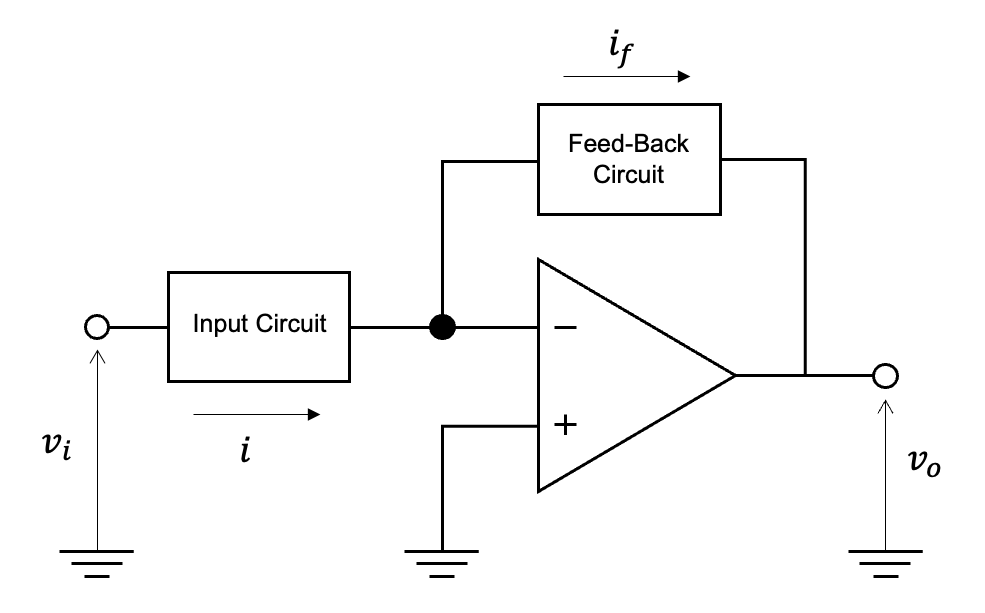
\includegraphics[width=7cm]{../image/di-base.png}
      \caption{OPアンプを用いた基本的な負帰還回路}
      \label{fig:di:base}
  \end{center}
\end{figure}
図\ref{fig:di:base}にOPアンプを用いた基本的な負帰還回路の構成を示す.
OPアンプは先述したとおり,OPアンプは外部に接続する素子を設計者が適切に選定することで線型な演算増幅を可能とするICである.
実際の設計においては,入力端子に特性を与える回路,負帰還の特性を与える回路をそれぞれ構成することとなる.

2つの回路中に使用する素子を変更することで,OPアンプはさまざまな電気的演算が可能となる.
R(抵抗)を用いる比例増幅・反転増幅をはじめ,R(抵抗)C(キャパシタ)を組み合わせ微・積分に対応できるほか,組み合わせ次第ではバンドパスフィルタやローパスフィルタなどのフィルタ回路も構成できる.

本実験では,反転増幅回路,微分・積分回路,バンドパスフィルタを扱う.

\paragraph{反転増幅回路\\}
図\ref{fig:di:case1}にOPアンプを用いた反転増幅回路を示す.
\begin{figure}[H]
  \begin{center}
      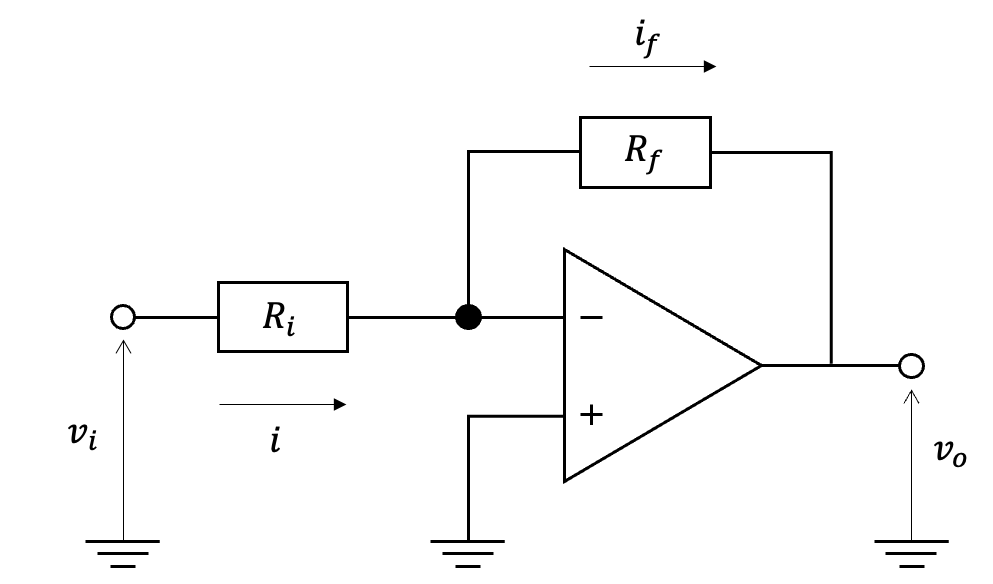
\includegraphics[width=7cm]{../image/di-case1.png}
      \caption{OPアンプを用いた反転増幅回路}
      \label{fig:di:case1}
  \end{center}
\end{figure}

反転増幅回路は,入力回路,負帰還回路にそれぞれR(抵抗)を用いて構成される.
OPアンプにはイマジナリーショートと呼ばれる特性があり,$\pm$入力端子が短絡した状態で安定する.
また,理想オペアンプにおいて入力端子のインピーダンスは$\infty$であることを考慮すれば,$i = i_f$である.

したがって,オームの法則より,$\frac{v_i}{R_i} = -\frac{v_0}{R_f}$が成り立つから
\begin{equation}
  v_{o} = -\frac{R_f}{R_i}v_i
\end{equation}

式より,入力電圧に対して出力電圧は$-R_f/R_i$倍となることがわかる.

\paragraph{微分回路\\}
図\ref{fig:di:case2}(a)にOPアンプを用いた微分回路を示す.
\begin{figure}[H]
  \centering
  \begin{minipage}{8cm}
    \centering
    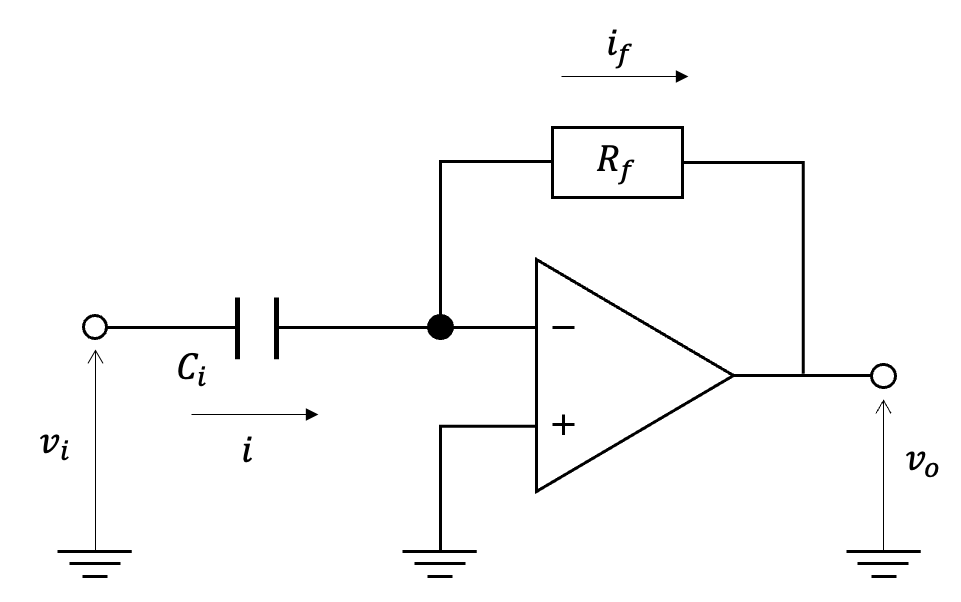
\includegraphics[keepaspectratio, scale=0.2]{../image/di-case21.png}
    \subcaption{微分回路}
  \end{minipage}
  \begin{minipage}{8cm}
    \centering
    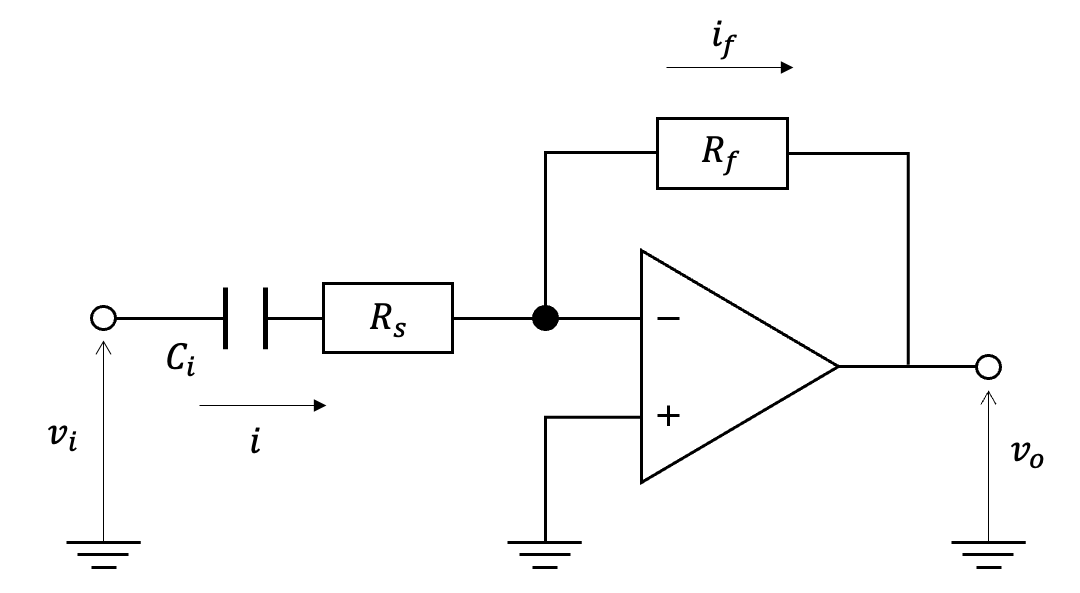
\includegraphics[keepaspectratio, scale=0.2]{../image/di-case22.png}
    \subcaption{実用微分回路}
  \end{minipage}
  \caption{OPアンプを用いた微分回路}
  \label{fig:di:case2}
\end{figure}

微分回路は反転増幅回路の入力回路をC(キャパシタ)に変更したものである.
C(キャパシタ)のインピーダンスは時間tに対して変動する.入力部のコンデンサ$C_i$に流れる電流は,$C_i\frac{dv}{dt}$であるから,
反転増幅回路と同様にオームの法則を適用すれば
\begin{eqnarray}
  C_i\frac{dv}{dt} &=& -\frac{v_0}{R_f}\\
  v_{o} &=& -C_i R_f\frac{dv}{dt}
\end{eqnarray}
という式が得られる.
これは,出力電圧が入力電圧の時間微分に比例することを示している.

しかしながら,C(キャパシタ)のインピーダンスは高周波領域においては低くなるため,入力が高周波になるほど入力電流が増大し,出力電圧が無限大に発散する.
OPアンプの駆動電圧は一般に$-15V \sim 15V$であり,出力電圧はこの時点で上限に達しクリッピングされるが,高周波ノイズを受けやすくなるため実用上は不適である.
このため一般的には図\ref{fig:di:case2}(b)に示すとおり,入力回路に$R_s$(抵抗)を挿入し,高周波領域において一定のインピーダンスを確保することで,出力電圧の発散を防ぐ実用微分回路が用いられる.

実用微分回路は入力信号が高周波に近づけば,$C_i$成分が無視できるようになり反転増幅回路と見做せるようになる.
$R_s$の効果が$C_i$成分を上回る点が,微分回路としての機能の限界であり,カットオフ周波数と呼ばれる.
カットオフ周波数は$R_s$と$C_i$の値に依存し,次式で求められる.
\begin{equation}
  f_{cut} = \frac{1}{2\pi R_s C_i}
\end{equation}

\paragraph{積分回路\\}
図\ref{fig:di:case3}(a)にOPアンプを用いた積分回路を示す.
\begin{figure}[H]
  \centering
  \begin{minipage}{8cm}
    \centering
    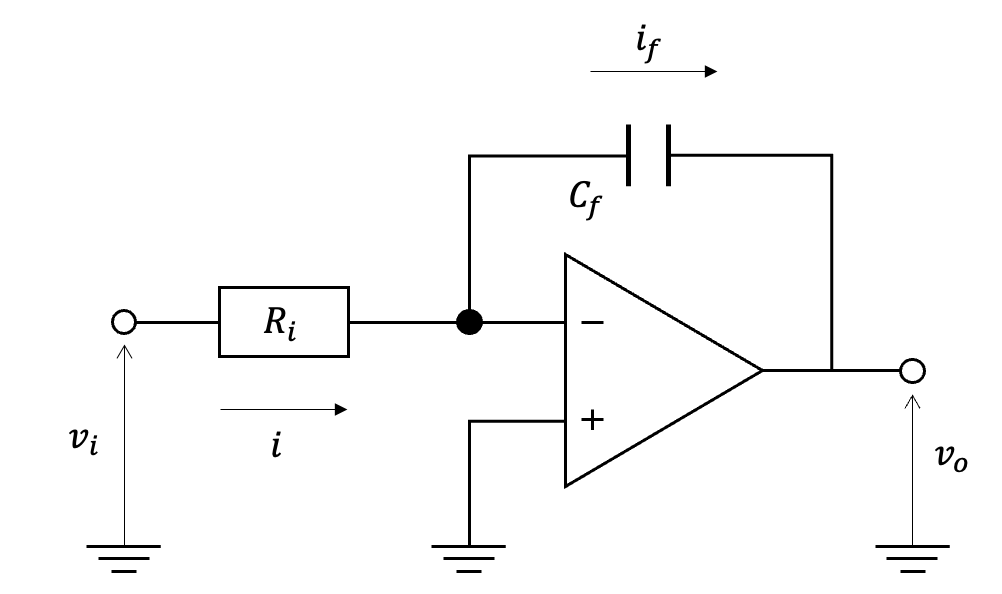
\includegraphics[keepaspectratio, scale=0.2]{../image/di-case31.png}
    \subcaption{積分回路}
  \end{minipage}
  \begin{minipage}{8cm}
    \centering
    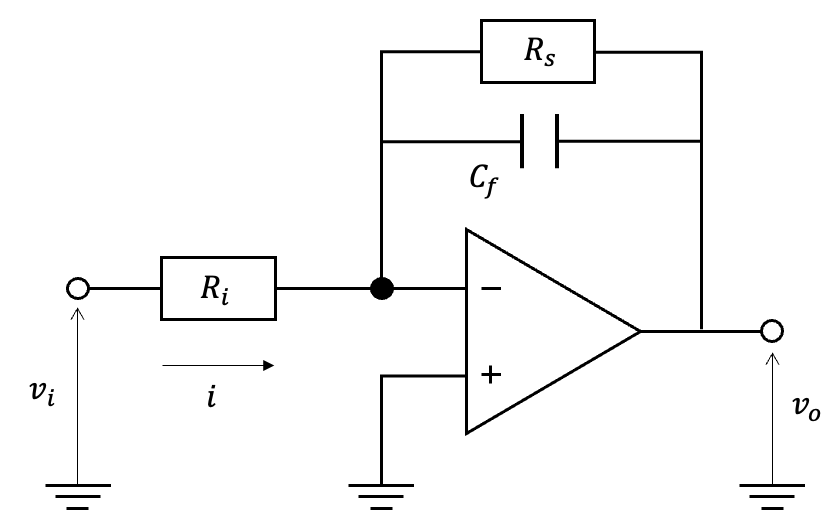
\includegraphics[keepaspectratio, scale=0.2]{../image/di-case32.png}
    \subcaption{実用積分回路}
  \end{minipage}
  \caption{OPアンプを用いた積分回路}
  \label{fig:di:case3}
\end{figure}

積分回路は反転増幅回路の負帰還回路をC(キャパシタ)に変更したものである.
微分回路と同様に
\begin{eqnarray}
  -v_o &=& \frac{1}{C_f}\int_0^t \frac{v_i}{R_i}dt\\
  v_o &=& -\frac{1}{R_i C_f}\int_0^t v_idt
\end{eqnarray}
となり,入力電圧が時間積分されることを示している.

回路内にコンデンサを使用しているため,低周波領域にてインピーダンス高くなり,出力が飽和する微分回路と酷似した問題を抱えているため,
実用上は図\ref{fig:di:case3}(b)に示すように,入力回路に$R_s$(抵抗)を挿入し,低周波領域において直流成分が通過可能な領域を確保することで,出力電圧の飽和を防ぐ実用積分回路が用いられる.
このとき,カットオフ周波数は同様に定義され,次式で求められる.
\begin{equation}
  f_{cut} = \frac{1}{2\pi R_s C_f}
\end{equation}

\paragraph{バンドパスフィルタ\\}
図\ref{fig:di:case4}にOPアンプを用いたバンドパスフィルタを示す.
\begin{figure}[H]
  \begin{center}
      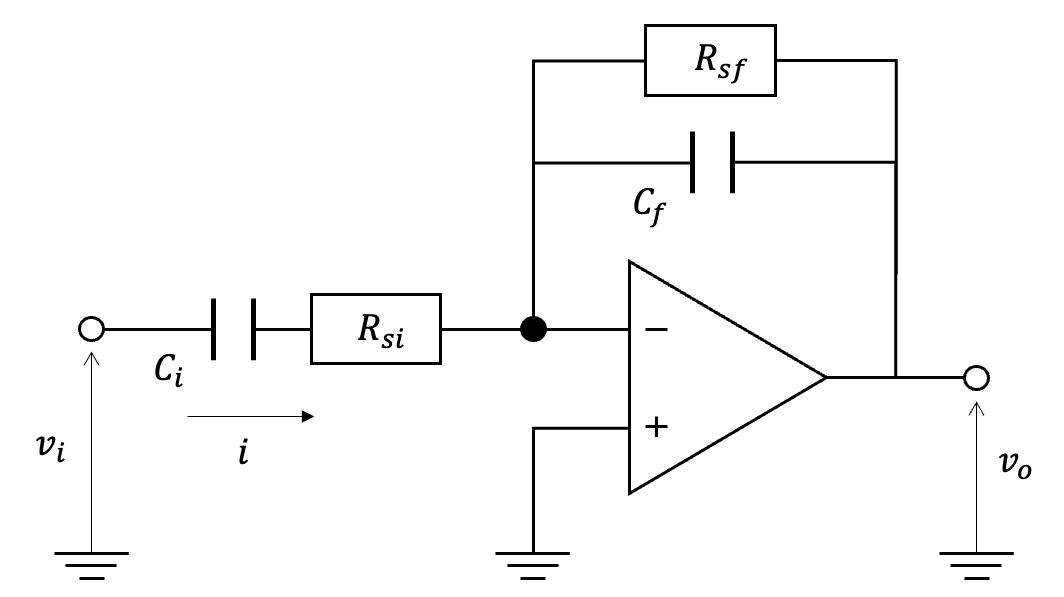
\includegraphics[width=7cm]{../image/di-case4.png}
      \caption{OPアンプを用いたバンドパスフィルタ}
      \label{fig:di:case4}
  \end{center} 
\end{figure}

バンドパスフィルタは,入力信号の特定の周波数帯域のみを通過させるフィルタである.
先に示した実用微分回路,実用積分回路はそれぞれ高周波領域,低周波領域においてインピーダンスの問題が生じ,出力電圧がカットオフされる特性があった.
これら2回路を組み合わせることで,2点のカットオフ周波数間の帯域の信号のみを通過するバンドパスフィルタを実現することができる.
一般的なバンドパスフィルタでは増幅の必要性はないため$R_{si} = R_{sf}$とし,利得0[dB]とする.

このときフィルタの動作は次のようになる.
\begin{eqnarray}
  \frac{v_o}{v_i} &=& \frac{\epsilon^{j\omega}}{\sqrt{ \{\frac{1}{R_{sf}^2}+(\omega C_f)^2\} \{R_si^2+(\omega C_i)^2\} } }
\end{eqnarray}
\begin{equation}
  \left( \phi = -arctan(\omega C_f R_{sf}) + arctan(\frac{1}{\omega C_i R_{si}}) \pm \pi \right) 
\end{equation}

\section{演算回路の動作観測}
\begin{figure}[H]
  \centering
  \begin{minipage}{8cm}
    \centering
    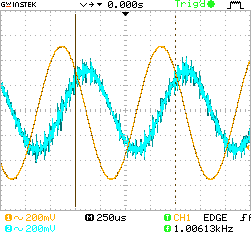
\includegraphics[keepaspectratio, scale=0.8]{../image/DS0000.png}
    \subcaption{正弦波入力に対する応答}
  \end{minipage}
  \begin{minipage}{8cm}
    \centering
    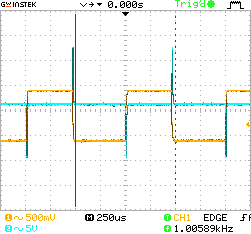
\includegraphics[keepaspectratio, scale=0.8]{../image/DS0001.png}
    \subcaption{矩形波入力に対する応答}
  \end{minipage}
  \caption{微分回路の動作波形}
  \label{fig:oc:case2}
\end{figure}

\begin{figure}[H]
  \centering
  \begin{minipage}{8cm}
    \centering
    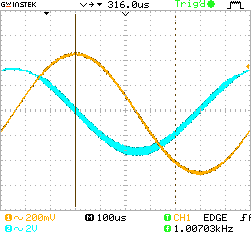
\includegraphics[keepaspectratio, scale=0.8]{../image/DS0002.png}
    \subcaption{正弦波入力に対する応答}
  \end{minipage}
  \begin{minipage}{8cm}
    \centering
    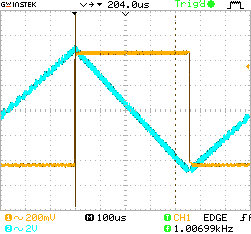
\includegraphics[keepaspectratio, scale=0.8]{../image/DS0003.png}
    \subcaption{矩形波入力に対する応答}
  \end{minipage}
  \caption{積分回路の動作波形}
  \label{fig:oc:case3}
\end{figure}

\section{演算回路の特性測定}
反転増幅回路(case 1),微分回路(case 2.1),実用微分回路(case 2.2),積分回路(case 3.1),実用積分回路(case 3.2),バンドパスフィルタ(case 4)とし,
各回路の閉ループ利得,入力に対する出力の位相差を測定する. 

\subsection{測定機器}
\paragraph{case 1}
\begin{enumerate}
  \item OPアンプ OP07
  \item ブレッドボード No.20
  \item 直流電源装置 TRACO POWER No.5
  \item 交流電源装置 KENWOOD AG-203 分類L151 帳1 番号99
  \item オシロスコープ GWINSTEK GDS-1022 No.19
\end{enumerate}

\paragraph{case 2 3 4}
\begin{enumerate}
  \item OPアンプ 5534D JRC
  \item ブレッドボード No.20
  \item 直流電源装置 TRACO POWER No.5
  \item 交流電源装置 KENWOOD AG-203 分類L151 帳1 番号99
  \item オシロスコープ GWINSTEK GDS-1022 No.19
\end{enumerate}

\subsection{使用定数}
\paragraph{case 1}
\begin{enumerate}
  \item $R_i$ 10k$\Omega$
  \item $R_f$ 20k$\Omega$
\end{enumerate}

\paragraph{case 4}
\begin{enumerate}
  \item $R_{is}$ 2k$\Omega$
  \item $R_{fs}$ 2k$\Omega$
  \item $C_{i}$ 10pF
  \item $C_{f}$ 1pF
\end{enumerate}

\subsection{測定内容・方法}
本実験では,演算回路に正弦波を入力し,周波数対閉ループ利得特性及び周波数対位相差特性を測定する.

\begin{figure}[H]
  \begin{center}
      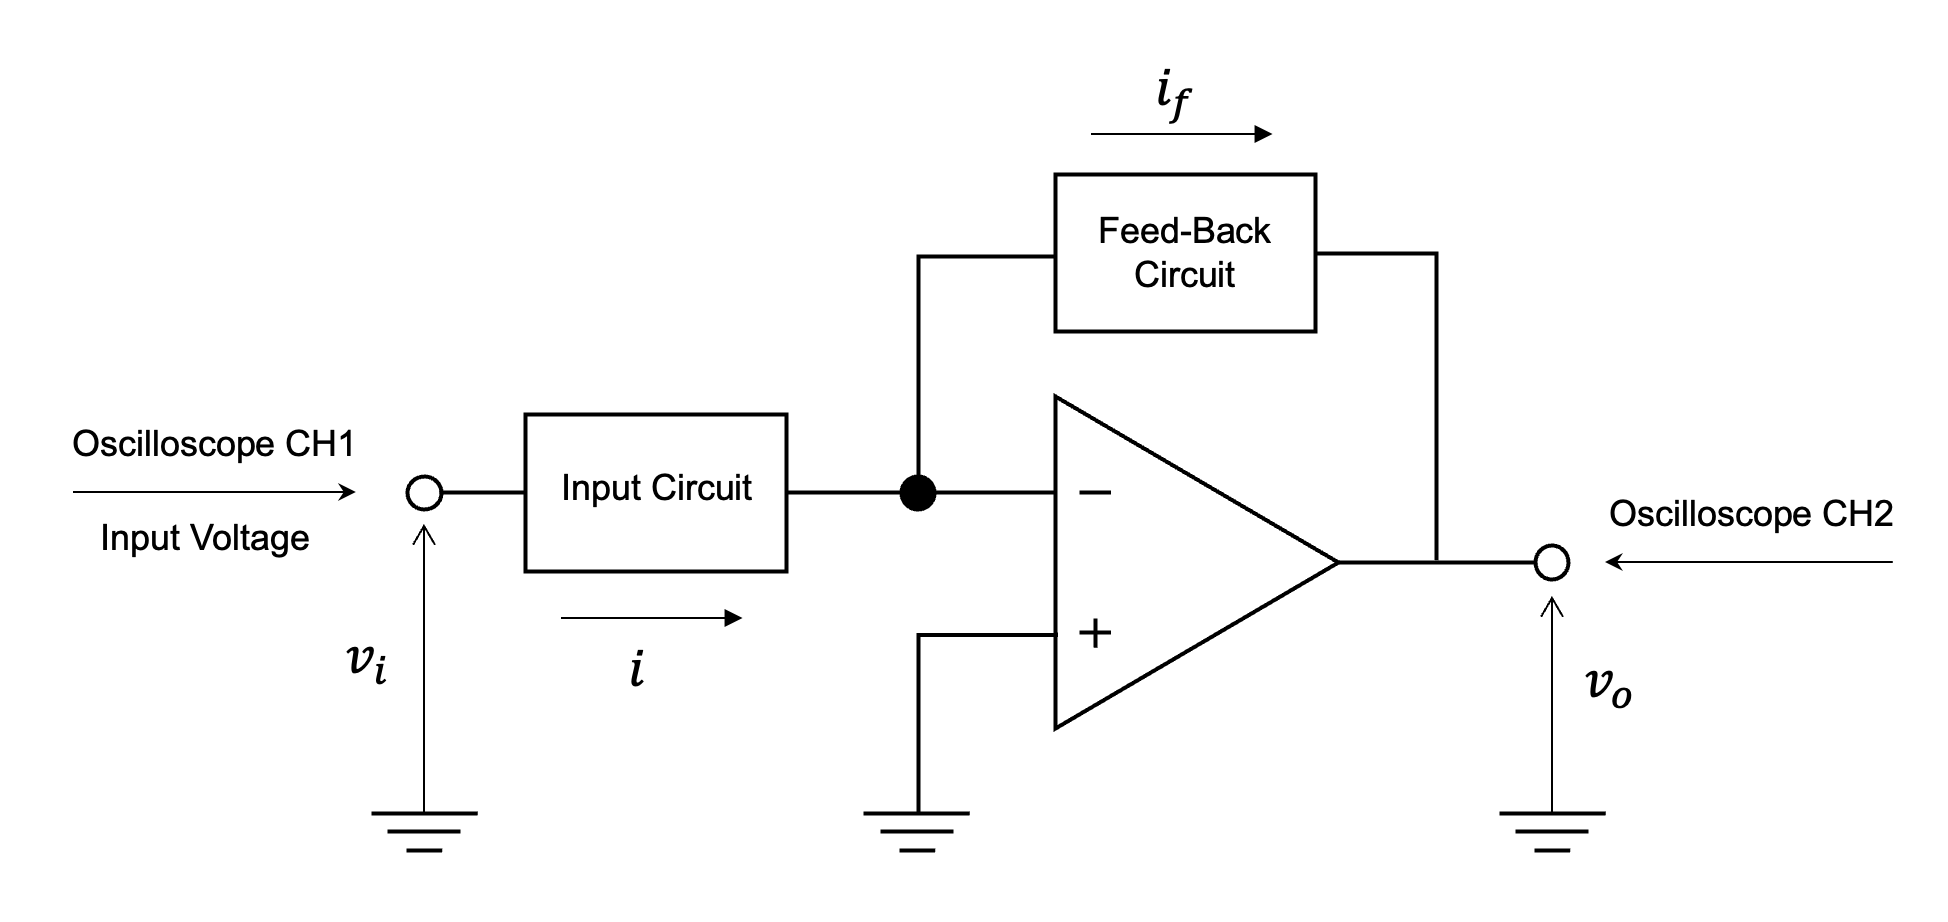
\includegraphics[width=8cm]{../image/dia-o.png}
      \caption{演算回路測定位置}
      \label{fig:di:o}
  \end{center}
\end{figure}
\paragraph{周波数対閉ループ特性}
演算回路に入力する正弦波の周波数を可変し,任意の周波数に対して回路が何[dB]増幅しているか測定する.
オシロスコープにて出力波形の振幅を目視にて確認し,必要な情報を記録する.

\paragraph{周波数対位相差特性}
演算回路に入力する正弦波の周波数を可変し,入力波形に対する出力波形の位相差を測定する.
オシロスコープにて位相差を目視確認し,必要な情報を記録する.

\subsection{case 1}
図\ref{fig:gr:case1}にcase 1の回路特性測定結果をグラフで示す.
\begin{figure}[H]
  \centering
  \begin{minipage}{8cm}
    \centering
    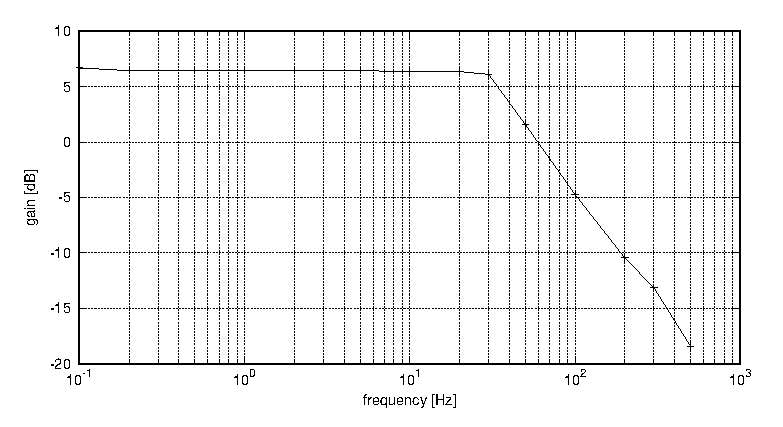
\includegraphics[keepaspectratio, scale=0.6]{../data/case1-g.eps}
    \subcaption{周波数対閉ループ利得特性}
  \end{minipage}
  \begin{minipage}{8cm}
    \centering
    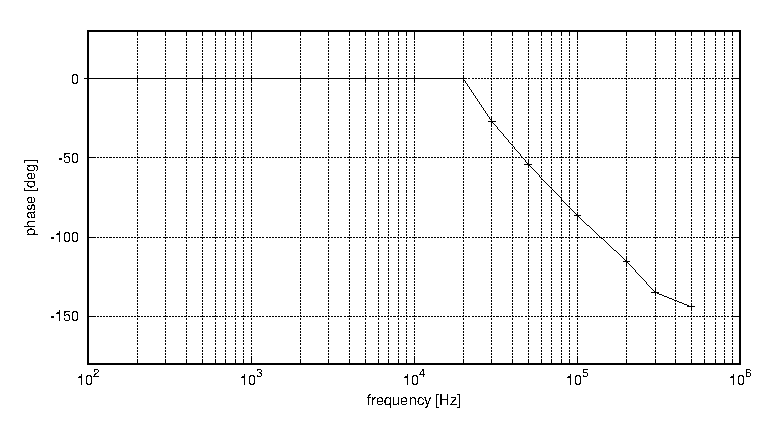
\includegraphics[keepaspectratio, scale=0.6]{../data/case1-f.eps}
    \subcaption{周波数対位相差特性}
  \end{minipage}
  \caption{case 1における回路特性測定結果}
  \label{fig:gr:case1}
\end{figure}

$R_i = 10k\Omega$ ,$R_f = 20k\Omega$より,測定対象の閉ループゲインは,次式で求められる.
\begin{eqnarray}
  G &=& 20 log_{10} \frac{R_f}{R_i}\\
  &=& 20 log_{10} \frac{20}{10}\\
  &\approx& 6.02 \mathrm{[Hz]}
\end{eqnarray}

また,非反転増幅回路にて位相差は発生しないため0である.

図\ref{fig:gr:case1}からは,$100$Hzから$20$kHz弱まではこの理論値を満たし,その後線形に降伏していることが確認できる.
この降伏は,オペアンプ内部に存在するC(キャパシタ)成分により,高周波領域において開ループゲインが減少することにより発生しているとみられる.

この特性が正しいか確認するため,文献[2]より,図\ref{fig:16}にOP07の閉ループ周波数応答特性を示す.
\begin{figure}[H]
  \begin{center}
      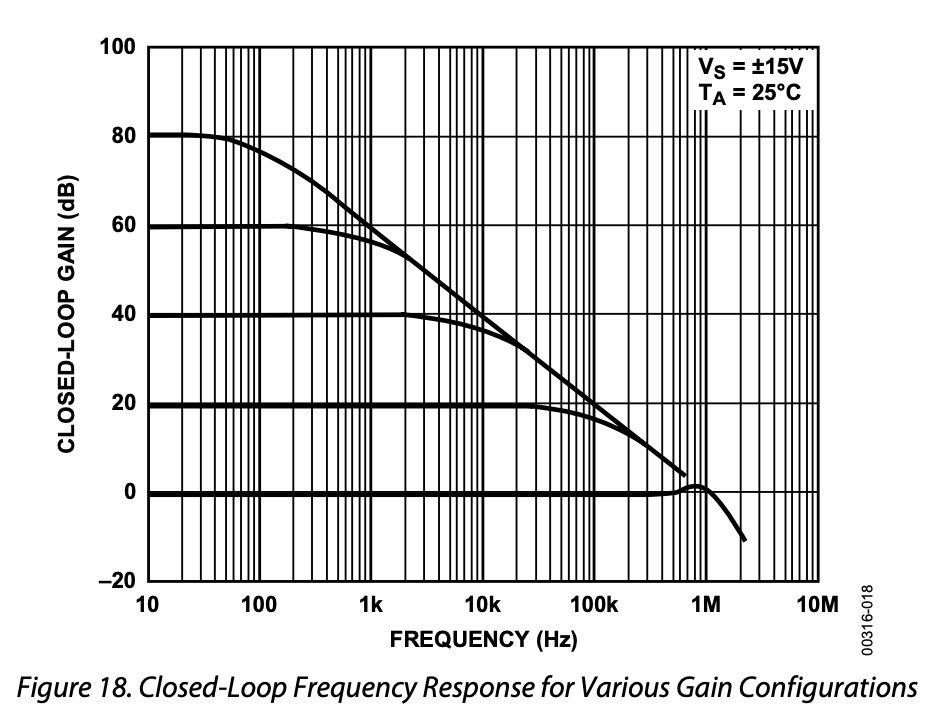
\includegraphics[width=7cm]{../image/fig16.png}
      \caption{データシート上の閉ループ周波数応答特性}
      \label{fig:16}
  \end{center}
\end{figure}
図\ref{fig:16}から,定常時の閉ループゲイン6[dB]として推定すると,10kHzから50kHzの間で降伏することがわかる.

また,LTSpice上でOP07アンプの特性を同様の回路を構成しシミュレーションを行ったところ,
図\ref{fig:gr:case1sim}に示す結果を得られた.
\begin{figure}[H]
  \centering
  \begin{minipage}{8cm}
    \centering
    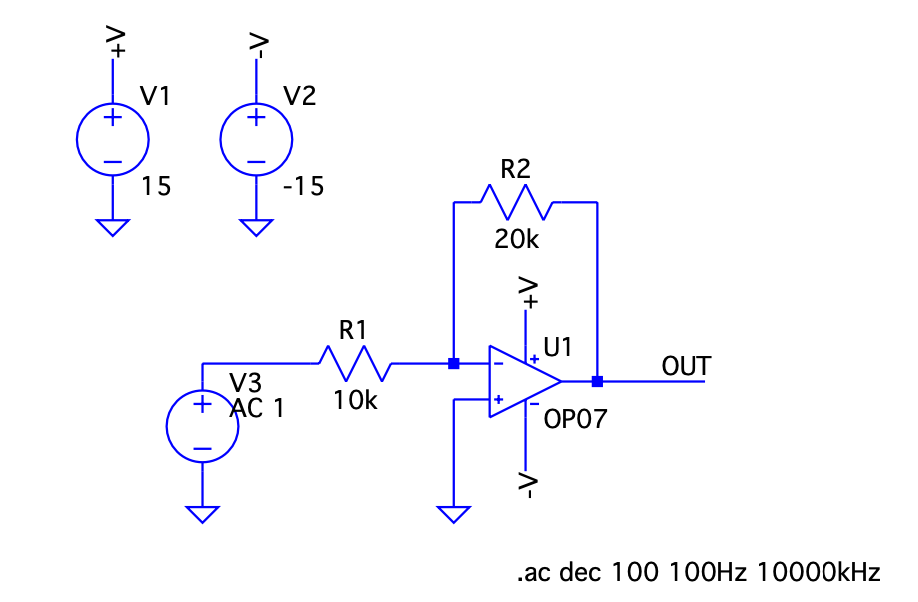
\includegraphics[keepaspectratio, scale=0.2]{../image/case1sim.png}
    \subcaption{構成したモデル}
  \end{minipage}
  \begin{minipage}{8cm}
    \centering
    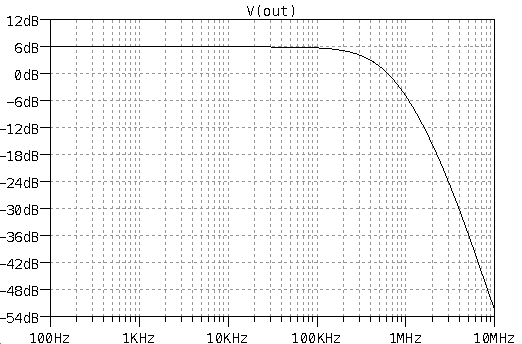
\includegraphics[keepaspectratio, scale=0.35]{../image/case1simout.png}
    \subcaption{シミュレーション結果}
  \end{minipage}
  \caption{LTSpiceを用いたcase 1のシミュレーション}
  \label{fig:gr:case1sim}
\end{figure}
この場合も,20kHz付近にて降伏が始まる様子が確認できる.

以上の結果から,測定値は正しい特性を観測したものであると判断する.

\subsection{case 2}
図\ref{fig:gr:case2}にcase 2.1 2.2の回路特性測定結果をグラフで重ねて示す.
\begin{figure}[H]
  \centering
  \begin{minipage}{8cm}
    \centering
    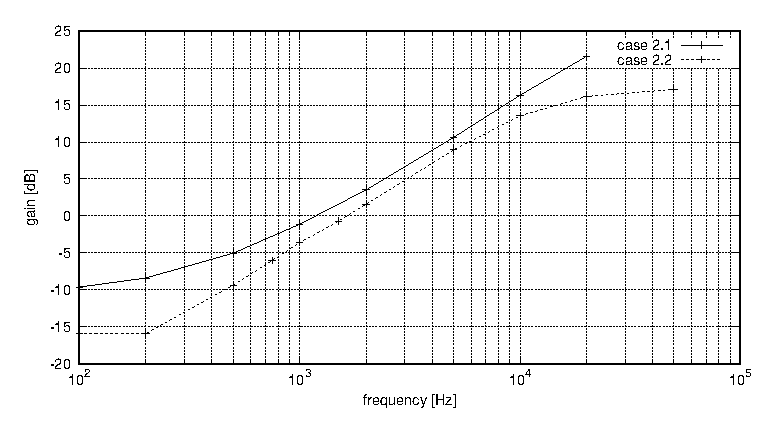
\includegraphics[keepaspectratio, scale=0.6]{../data/case2-g.eps}
    \subcaption{周波数対閉ループ利得特性}
  \end{minipage}
  \begin{minipage}{8cm}
    \centering
    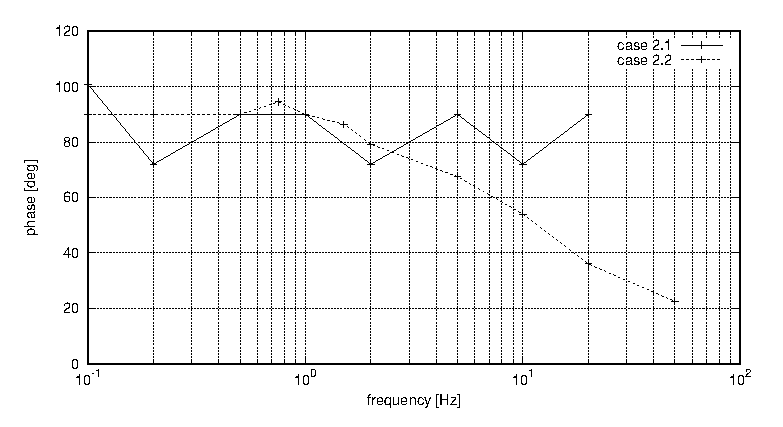
\includegraphics[keepaspectratio, scale=0.6]{../data/case2-f.eps}
    \subcaption{周波数対位相差特性}
  \end{minipage}
  \caption{case 2.1 2.2における回路特性測定結果}
  \label{fig:gr:case2}
\end{figure}

図\ref{fig:gr:case2}(a)の高周波領域おいて,case 2.2がcase 2.1に対して線形性を失い,増幅率が下がっていることから,$R_s$による
インピーダンス補償が働いていることが観察できる.
また,図\ref{fig:gr:case2}(b)では,case 2.1が位相差+90deg程度の特性を示しており,入力波形に対して
微分されていることがわかる.一方case 2.2は周波数の増加に伴い,微分回路としての特性が失われ反転増幅回路に近づくため,
位相差が0degに向かって減少している.

ここで,カットオフ周波数$f_{cut}$とすると,
\begin{eqnarray}
  f_{cut} &=& \frac{1}{2\pi R_s C_i}\\
  &\approx& 6.02 \mathrm{[Hz]}
\end{eqnarray}

\subsection{case 3}
図\ref{fig:gr:case3}にcase 3.1 3.2の回路特性測定結果をグラフで重ねて示す.
\begin{figure}[H]
  \centering
  \begin{minipage}{8cm}
    \centering
    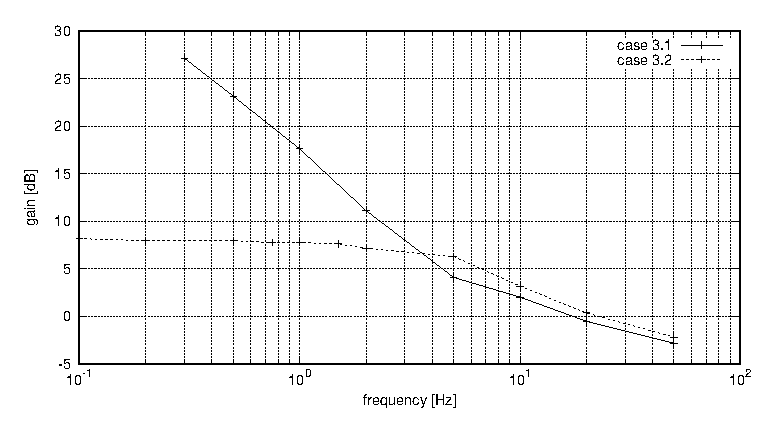
\includegraphics[keepaspectratio, scale=0.6]{../data/case3-g.eps}
    \subcaption{周波数対閉ループ利得特性}
  \end{minipage}
  \begin{minipage}{8cm}
    \centering
    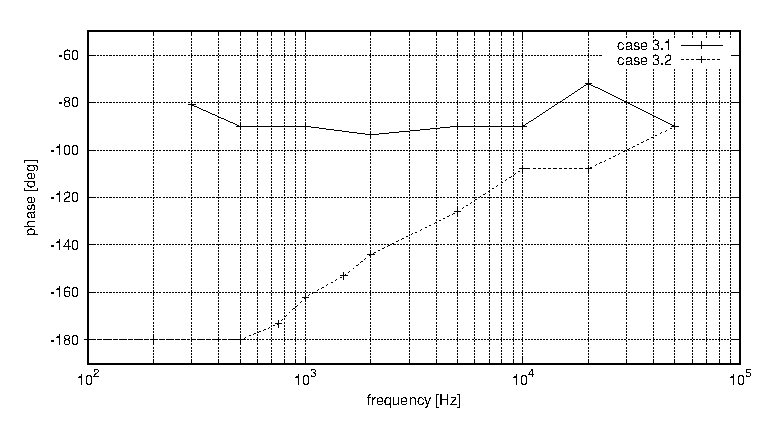
\includegraphics[keepaspectratio, scale=0.6]{../data/case3-f.eps}
    \subcaption{周波数対位相差特性}
  \end{minipage}
  \caption{case 3.1 3.2における回路特性測定結果}
  \label{fig:gr:case3}
\end{figure}

図\ref{fig:gr:case3}(a)の低周波領域おいて,case 3.2がcase 3.1に対して線形性を失い,増幅率が下がっていることから,$R_s$による
インピーダンス補償が働いていることが観察できる.
また,図\ref{fig:gr:case3}(b)では,case 3.1が位相差-90deg程度の特性を示しており,入力波形に対して
積分されていることがわかる.case 3.2は周波数の増加に伴って実用微分回路としての特性が大きくなるため,-90degに近づく特性となっている,

カットオフ周波数は,
\begin{eqnarray}
  f_{cut} &=& \frac{1}{2\pi R_s C_f}\\
  &\approx& 6.02 \mathrm{[Hz]}
\end{eqnarray}

\subsection{case 4}
図\ref{fig:gr:case4}にcase 4の回路特性測定結果をグラフで示す.
\begin{figure}[H]
  \centering
  \begin{minipage}{8cm}
    \centering
    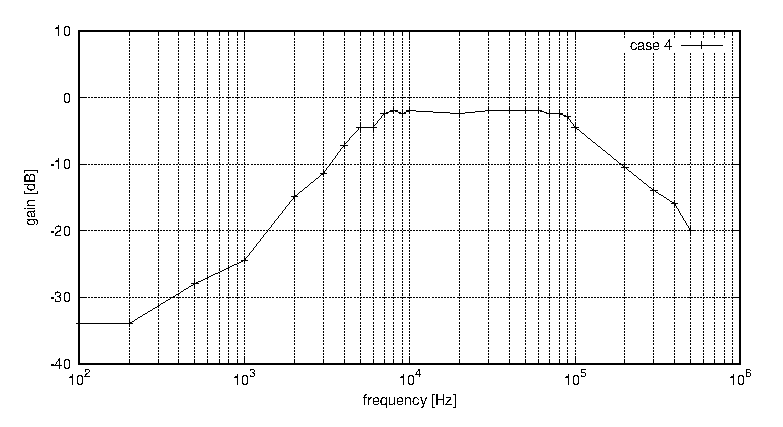
\includegraphics[keepaspectratio, scale=0.6]{../data/case4-g.eps}
    \subcaption{周波数対閉ループ利得特性}
  \end{minipage}
  \begin{minipage}{8cm}
    \centering
    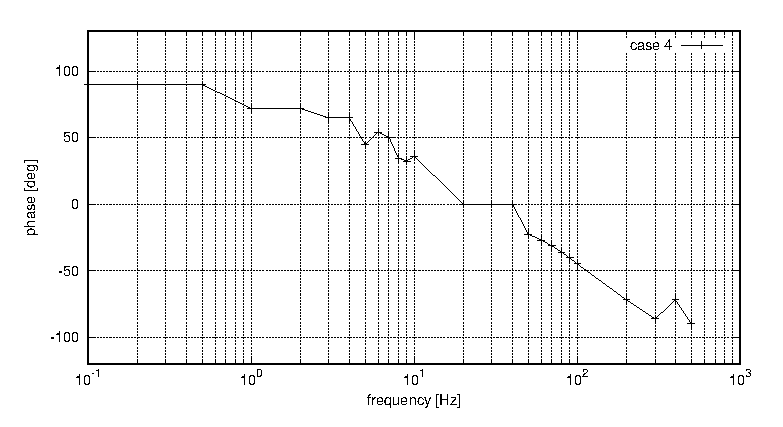
\includegraphics[keepaspectratio, scale=0.6]{../data/case4-f.eps}
    \subcaption{周波数対位相差特性}
  \end{minipage}
  \caption{case 4における回路特性測定結果}
  \label{fig:gr:case4}
\end{figure}

図\ref{fig:gr:case3}(a)から,低周波,高周波領域にてゲインが低下し,特定の帯域のみ通過(0db)しているバンドパスフィルタの特性が確認できる.
図\ref{fig:gr:case3}(b)では実用微分回路による位相変動が顕著にみられる,より高周波の領域にて-90degに漸近することが推定される.

低域カットオフ周波数$f_{Lcut}$,高域カットオフ周波数$f_{Hcut}$とすると,
\begin{eqnarray}
  f_{Lcut} &=& \frac{1}{2\pi R_s C_i}\\
  &\approx& 7960 \mathrm{[Hz]}
\end{eqnarray}
\begin{eqnarray}
  f_{Hcut} &=& \frac{1}{2\pi R_s C_f}\\
  &\approx& 79600 \mathrm{[Hz]}
\end{eqnarray}

これら帯域特性は測定データと合致する.
したがって測定値は正しい特性を観測したものだと判断する.

\section{付録 測定データ}

\begin{thebibliography}{99}
  \bibitem{ataka} 永井 誠、実験テキスト「OPアンプの基礎・応用」、(2022年)
  \bibitem{ad} Analog Devices、OP07 Deta Sheet、https://www.analog.com/media/en/technical-documentation/data-sheets/OP07.pdf、(accessed 2022/12)
\end{thebibliography}

\end{document}